% options:
% thesis=B bachelor's thesis
% thesis=M master's thesis
% czech thesis in Czech language
% english thesis in English language
% hidelinks remove colour boxes around hyperlinks

\documentclass[thesis=B,english]{FITthesis}[2012/10/20]

% \usepackage[utf8]{inputenc} % LaTeX source encoded as UTF-8
% \usepackage[latin2]{inputenc} % LaTeX source encoded as ISO-8859-2
% \usepackage[cp1250]{inputenc} % LaTeX source encoded as Windows-1250

\usepackage{graphicx} %graphics files inclusion
% \usepackage{subfig} %subfigures
% \usepackage{amsmath} %advanced maths
% \usepackage{amssymb} %additional math symbols

\usepackage{dirtree} %directory tree visualisation

% % list of acronyms
% \usepackage[acronym,nonumberlist,toc,numberedsection=autolabel]{glossaries}
% \iflanguage{czech}{\renewcommand*{\acronymname}{Seznam pou{\v z}it{\' y}ch zkratek}}{}
% \makeglossaries

% % % % % % % % % % % % % % % % % % % % % % % % % % % % % % 
% EDIT THIS
% % % % % % % % % % % % % % % % % % % % % % % % % % % % % % 
\setcounter{tocdepth}{2}
\department{Department of Software Engineering}
\title{Adobe Premiere Pro Plugin for NARRA}
\authorGN{Dmitry} %author's given name/names
\authorFN{Vanyagin} %author's surname
\author{Dmitry Vanyagin} %author's name without academic degrees
\authorWithDegrees{Dmitry Vanyagin} %author's name with academic degrees
\supervisor{Petr Pulc}
\acknowledgements{THANKS}
\abstractEN{Summarize the contents and contribution of your work in a few sentences in English language.}
\abstractCS{V n{\v e}kolika v{\v e}t{\' a}ch shr{\v n}te obsah a p{\v r}{\' i}nos t{\' e}to pr{\' a}ce v {\v c}esk{\' e}m jazyce.}
\placeForDeclarationOfAuthenticity{Prague}
\keywordsCS{Replace with comma-separated list of keywords in Czech.}
\keywordsEN{Replace with comma-separated list of keywords in English.}
\declarationOfAuthenticityOption{1} %select as appropriate, according to the desired license

\graphicspath{ {./IMAGES/} }

\begin{document}

% \newacronym{CVUT}{{\v C}VUT}{{\v C}esk{\' e} vysok{\' e} u{\v c}en{\' i} technick{\' e} v Praze}
% \newacronym{FIT}{FIT}{Fakulta informa{\v c}n{\' i}ch technologi{\' i}}

\setsecnumdepth{part}
\chapter{Introduction}
The possibility to visualize and annotate data is always been appreciated in circles of people, who works with a huge amounts of information every day. NARRA is a software that provides this functionality for those using large amounts of video in their practice – artists collaborating on open narratives, video editors, social scientists using video as a research tool, documentary filmmakers with expanded projects. 

Artists can tell stories together using video. Instead of a linear narrative, media works can have multiple paths, multiple versions. The software can be used to create, visualize and navigate a tree of linked stories.

Video editors faced with hundreds of hours of material can annotate their media objects and then organize it based on complex search categories. The software itself will use existing software libraries to add functionality and perform automated annotations. For example the software can extract spoken words and make them into attached text; list shot size, geographic location, etc.

The main purpose of this thesis is to create a tool to use all this functionality and communicate with NARRA directly from your computer. I chose to implement it as a plug-in for Adobe Premiere Pro video editing software application. This application is widely used by different broadcasters such as the BBC\cite{bbc} and CNN\cite{cnn}, also many people chose it as a part or their workflow. Using this plug-in user will be able to directly communicate with NARRA API, i.e., to import and export sequences of clips with all attached metadata. 

To develop this tool I will use mainly Adobe Premiere Pro SDK and Third-party libraries for solving arising problems or for extending functionality provided by SDK.
\chapter{Analysis and Design}
\section{Requirements specification}
\subsection{Functional requirements}
Final product have to fulfill basic requirements:
	\begin{description}
		\item [Authorization in NARRA] 
User should be able to authorize in NARRA, get a token that will be used for all transactions between plug-in and NARRA API. Since Google identities are used inside NARRA, plug-in should communicate with Google authorization services.
		\item [Displaying a list of uploaded projects]
User should be able to browse a list of his projects that he exported to NARRA.
		\item [Searching a project by name]
Plug-in should provide convenient search input field for a user to search in a project list.
		\item [Importing a project from NARRA to Adobe Premiere Pro]
User should be able to choose a project from his project list and import it in the Adobe Premiere Pro.
		\item [Exporting a new project from Adobe Premiere Pro to NARRA]
User should be able to export a new project from Adobe Premiere Pro to NARRA.
		\item [Pushing changes of a project to NARRA]
User should be able to synchronize all changes made in project with NARRA.
		\item [Synchronization of project metadata between NARRA and local machine]
Plug-in should support synchronization of project metadata between NARRA and Adobe Premiere Pro project.
	\end{description}
\subsection{Non-Functional requirements}
	\begin{itemize}
		\item User interface should be clear and understandable for a user.
		\item Plug-in should estimate the length operations and provide a visual representation (progress bars)
		\item Plug-in should work in Adobe Premiere Pro CS5.5 and newer versions.
		\item Internet connection is required to use all functionality.
	\end{itemize}
\section{Use cases}
In this section I will try to describe the basic use cases for this application. In order to communicate with NARRA, user has to complete authorization process, that's why almost every use case require user to be logged in. You can see use case diagram on figure \ref{fig:usecase}.
	\begin{description}
		\item[Authorization in NARRA] 
User wants to authorize himself in order to use plug-in. Authorization process is carried out by Google.
		\item[Browsing project list] 
User can see a list of his/her projects exported to NARRA. He/she is able to scroll the list, select a project. Requirements: User has to be logged in. 
		\item[Import new project from NARRA]
User wants to import a project from NARRA. Project is selected from a list, after double click on the project, importing process starts, user sees progress bar of the import. Requirements: User has to be logged in. 
		\item[Export project to NARRA]
User wants to export a project to NARRA. Current project in Adobe Premiere Pro will be pushed to NARRA after successful launch. User sees progress bar of export process with time estimation. Requirements: User has to be logged in.
		\item[Editing of metadata]
User wants to edit project metadata and save changes back to NARRA. User can add metadata using Adobe Premiere Pro tools. Requirements: User has to be logged in.
		\item[Searching for a project]
User wants to find a project in his project list. Name of the project should be written in a search box. List of projects will be automatically refreshed after each letter typed in search box. Requirements: User has to be logged in.
	\end{description}
	\begin{figure}
		\centering
		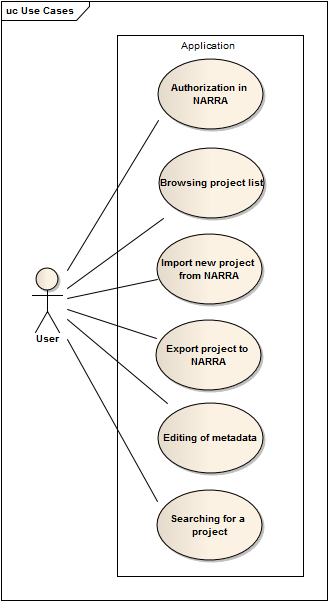
\includegraphics[width=0.7\textwidth]{UseCases.png}
		\caption{Use case diagram}\label{fig:usecase}
	\end{figure}
\section{Structure of application}
I decided to split this application into two plug-ins:
	\begin{itemize}
		\item Import plug-in (Importer).
		\item Export plug-in (Exporter).
	\end{itemize}
The reason why I chose this structure is because it is more logical to have two lightweight plug-ins that solve it's own task. If user wants to import a project into Adobe Premiere Pro, he/she can launch Importer, to export a project Exporter can be used. On figure \ref{fig:narrastruct} you can see a sketch of communication between application and NARRA, you can see that plug-in directly uses Adobe Premiere Pro SDK and communicates with NARRA using http requests. All video files are stored in a cloud storage.
	\begin{figure}
		\centering
		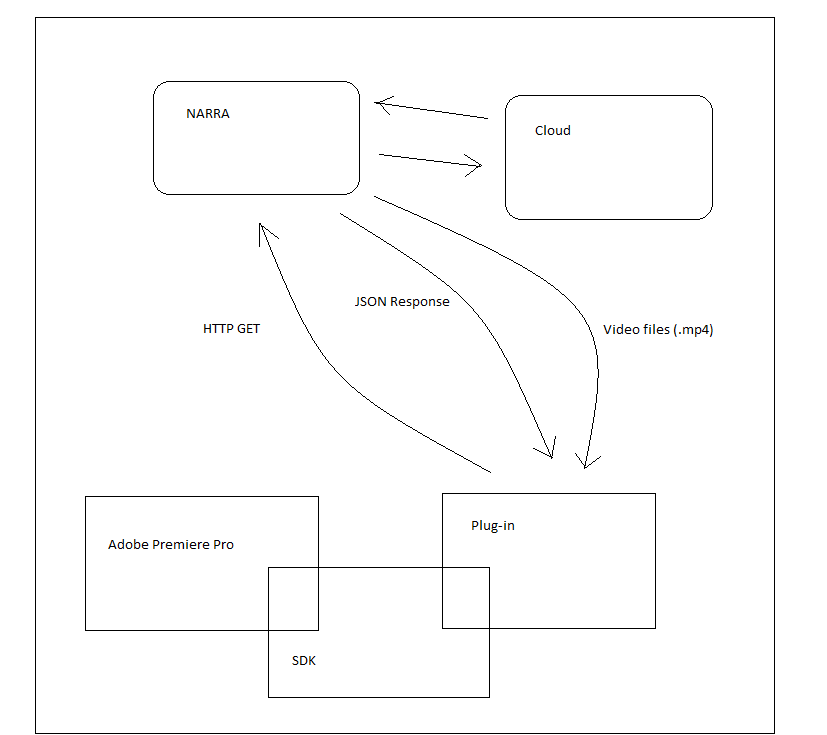
\includegraphics[width=1\textwidth]{StructureofNARRA.png}
		\caption{Sketch of communication with NARRA}\label{fig:narrastruct}
	\end{figure}
\section{Authorization}
To communicate with NARRA, user has to be authorized. NARRA uses google identities as a user objects, that is the reason why I have to somehow embed Google authorization service into this plug-in. I decided to do by using a web browser and login form provided by Google. Basic scenarion will be like this:
	\begin{enumerate}
		\item User launches plug-in.
		\item Browser window opens up and request is sent to Google to start authorization process.
		\item User sees Google login form.
		\item User enters his/her username and password and allows plug-in to use profile data.
		\item Plug-in receives token that will be used for communication with NARRA.
	\end{enumerate}
\subsection{OAuth 2.0}
OAuth is an open standard for authorization. OAuth provides client applications a "secure delegated access" to server resources on behalf of a resource owner. It specifies a process for resource owners to authorize third-party access to their server resources without sharing their credentials. 

Designed specifically to work with Hypertext Transfer Protocol (HTTP), OAuth essentially allows access tokens to be issued to third-party clients by an authorization server, with the approval of the resource owner, or end-user. The client then uses the access token to access the protected resources hosted by the resource server. OAuth is commonly used as a way for web surfers to log into third party web sites using their Microsoft, Google, Facebook or Twitter accounts, without worrying about their access credentials being compromised.\cite{oauth}

In order to use OAuth 2.0, the installed application must either have access to the system browser, or it must have a browser embedded as a web view. The OAuth 2.0 flow for installed applications is as follows:
	\begin{enumerate}
		\item Your application redirects a browser to a Google URL. The URL query parameters indicate the type of Google API access that the application requires.
		\item As in other scenarios, Google handles user authentication and consent, and the result of the sequence is an authorization code. The authorization code is returned in the title bar of the browser or as a query string parameter, depending on the parameters your application sends in the request.
		\item Your application exchanges the authorization code for an access token and a refresh token. During this exchange, the application presents its client ID and client secret that is obtained from the Developers Console.
		\item Your application uses the access token to make calls to a Google API and stores the refresh token for future use.\cite{oauthdesc}
	\end{enumerate}
As we can see from OAuth web flow (figure \ref{fig:oauth}), authorization process goes in two steps, I need to somehow do it in a way that is convenient for a user. I decided to start this process by pressing a button, request token will be formed automatically and sent to Google. Second task is to figure out how to get authorization code to our application in order to exchange it for an access token later. One way is to make user to enter authorization code to the application (that will be displayed in browser window after user provide his/her credentials and agrees that our plug-in will use profile information), second way is to get this code as part of the query string that is sent to localhost.\cite{oauthdesc}

Parameters that are interesting for us to form request token:
	\begin{description}
		\item[redirect\_uri] 
Determines where the response is sent. The value of this parameter must exactly match one of the values that appear in the Credentials page in the Google Developers Console (including the http or https scheme, case, and trailing slash). You may choose between urn:ietf:wg:oauth:2.0:oob, urn:ietf:wg:oauth:2.0:oob:auto, or an http://localhost port. Value of this parameter will determine the way of getting authorization code that we will exchange for an access token.
		\item[client\_id] 
Identifies the client that is making the request. The value passed in this parameter must exactly match the value shown in the Google Developers Console.
	\end{description}

	\begin{figure}
		\centering
		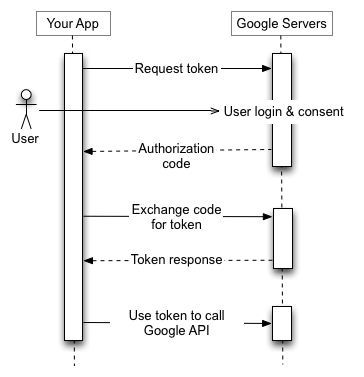
\includegraphics[width=0.7\textwidth]{oauthwebflow.png}
		\caption{OAuth web flow}\label{fig:oauth}
	\end{figure}

\section{NARRA}

\subsection{NARRA API}
\chapter{Adobe Premiere Pro}
\section{Overview}

Adobe Premiere Pro is a timeline-based video editing software application. It is part of the Adobe Creative Cloud, which includes video editing, graphic design, and web development programs.

Premiere Pro has been used to edit feature films, such as Gone Girl, Captain Abu Raed, and Monsters, and other venues such as Madonna's Confessions Tour.\cite{adobe}

	\begin{figure}
		\centering
		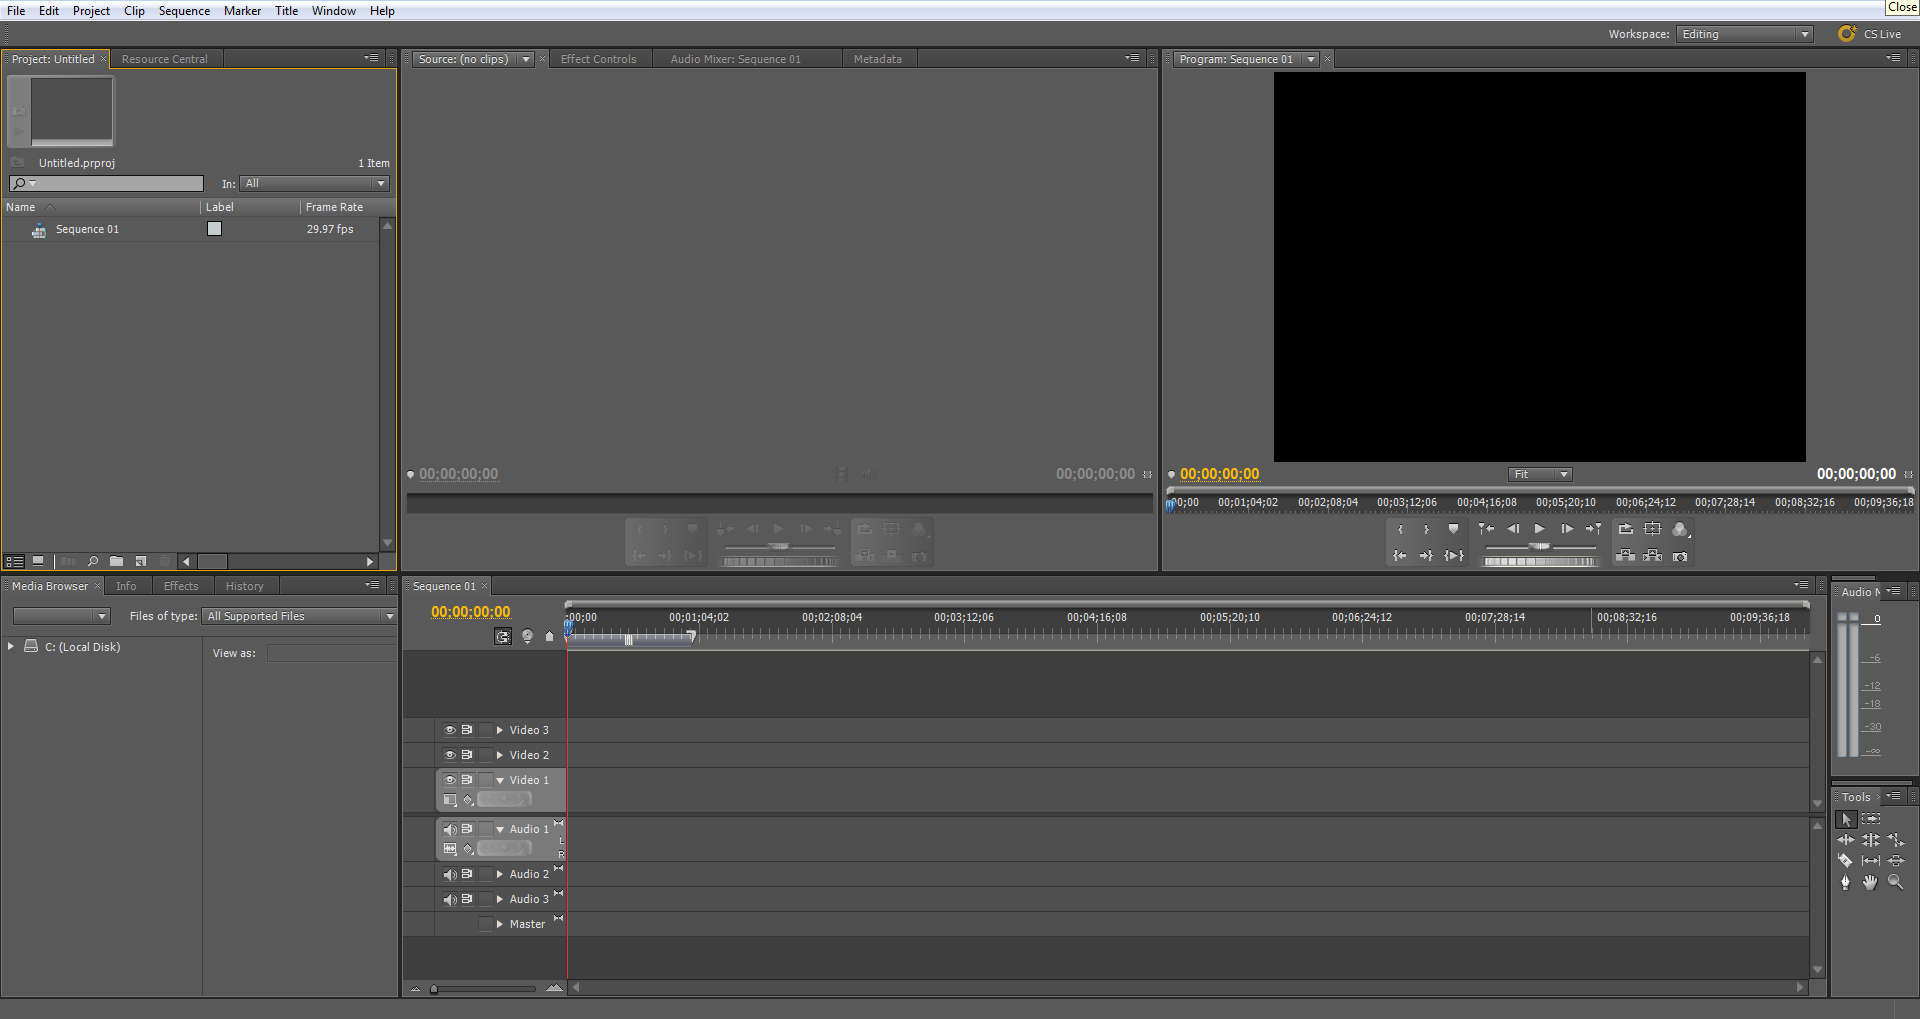
\includegraphics[width=0.8\textwidth]{PremiereMain.png}
		\caption{Adobe Premiere Pro CS5.5 window}\label{fig:APPWindow}
	\end{figure}

\section{History}

Premiere Pro is the redesigned successor to Adobe Premiere, and was launched in 2003. Premiere Pro refers to versions released in 2003 and later, whereas Premiere refers to the earlier releases. Premiere was one of the first computer-based NLEs (non-linear editing system), with its first release on Mac in 1991. Up until version Premiere Pro 2.0 (CS2), the software packaging featured a galloping horse, in a nod to Eadweard Muybridge's work, "Sallie Gardner at a Gallop".\cite{adobe}

\section{Software Development Kit}
The Adobe Premiere Pro plug-in and software development kits (SDK) allow us to build plug-ins to enhance and extend the capabilities of Premiere Pro. I will use it's functionality to implement sequence importer and exporter.
\subsection{Importer}
Importers provide video and/or audio from the media source. This source can be a single file, a set of files, a communication link between another application, etc.
\subsection{Exporter}

\chapter{Analysis}

\section{Requirements}

\section{Communication with NARRA API}
In order to communicate with NARRA RESTful API in C++ I had to find a library or framework, because language itself doesn't provide any methods to work with http protocol. I chose libcurl library, because it is lightweight and effective.
\subsection{Libcurl}
Libcurl 


\chapter{Implementation}

\setsecnumdepth{part}
\chapter{Conclusion}


\bibliographystyle{iso690}
\bibliography{Bibliography}

\setsecnumdepth{all}
\appendix

\chapter{Acronyms}
% \printglossaries
\begin{description}
	\item[GUI] Graphical user interface
	\item[XML] Extensible markup language
\end{description}


\chapter{Contents of enclosed CD}

%change appropriately

\begin{figure}
	\dirtree{%
		.1 readme.txt\DTcomment{the file with CD contents description}.
		.1 exe\DTcomment{the directory with executables}.
		.1 src\DTcomment{the directory of source codes}.
		.2 wbdcm\DTcomment{implementation sources}.
		.2 thesis\DTcomment{the directory of \LaTeX{} source codes of the thesis}.
		.1 text\DTcomment{the thesis text directory}.
		.2 thesis.pdf\DTcomment{the thesis text in PDF format}.
		.2 thesis.ps\DTcomment{the thesis text in PS format}.
	}
\end{figure}

\end{document}
